\chapter{Condizionamento dell'Ingresso}

%--------------------------------------------------------------------------------------------

\section{Convertitore Lineare-Esponenziale}

%--------------------------------------------------------------------------------------------

Vogliamo ora analizzare il circuto che soddisfa la specifica sulla modalità $1\ V/Octave$
dell'ingresso, ovvero il circuito in grado di convertire una tensione lineare in una
esponenziale.

Il circuito utilizzato è molto diffuso in questo tipo di applicazioni, si può infatti
trovare in molti siti di DIY come quello di René Schmitz \cite{expo_converter}, personaggio
molto noto tra gli appassionati di sintetizzatori musicali fai-da-te.

%--------------------------------------------------------------------------------------------

\subsection*{Analisi del Circuito}

%--------------------------------------------------------------------------------------------

Per l'applicazione si sfrutta la caratteristica esponenziale intrinseca del transistor
bipolare, ovvero:

\begin{displaymath}
    I_e\approx I_c=I_se^{\left(\frac{V_{be}}{V_T}-1\right)}
    \approx I_se^{\left(\frac{V_{be}}{V_T}\right)}\ [A]
\end{displaymath}

\begin{figure}[H]
    \centering
    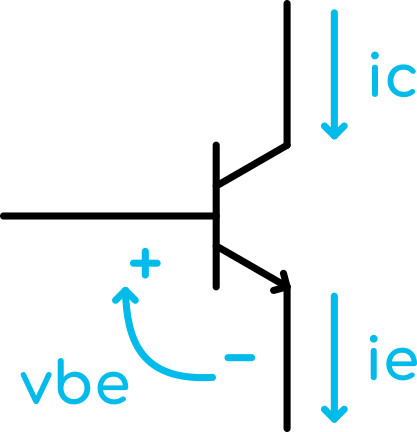
\includegraphics{circuits/single_transistor_circuit.png}
    \caption{BJT}
    \label{bjt}
\end{figure}

dove $V_T$ (o potenziale termico) e $I_s$ (o corrente di saturazione) sono variabili in
funzione della temperatura. Nella nostra analisi $V_T$ verrà considerato di valore costante
pari a $26\ mV$, mentre si rimuove dall'equazione $I_s$ collegando una coppia di transistor
(idealmente nello stesso chip, in modo che siano il più possibile simili tra loro e ù
termicamente accoppiati) in configurazione differenziale:

\begin{figure}[H]
    \centering
    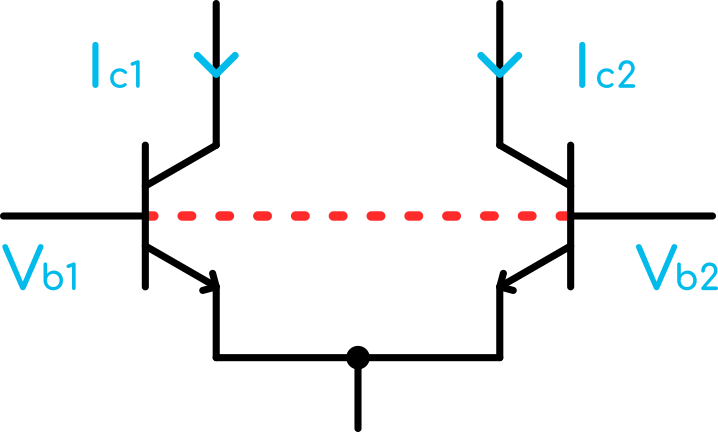
\includegraphics{circuits/differential_pair_circuit.png}
    \caption{Coppia differenziale a BJT}
    \label{differential_pair_circuit}
\end{figure}

per la quale possiamo scrivere la seguente relazione:

\begin{displaymath}
    \frac{I_{c2}}{I_{c1}}=\frac{I_s e^{\left(\frac{V_{be2}}{V_T}\right)}}{I_s e^{\left(\frac{V_{be1}}{V_T}\right)}}
    \qquad
    \rightarrow
    \qquad
    I_{c2}=I_{c1}e^{\left(\frac{V_{be2}-V_{be1}}{V_T}\right)}=I_{c1}e^{\left(\frac{V_{b2}-V_{b1}}{V_T}\right)}\ [A]
\end{displaymath}

in cui risulta evidente che la dipendenza da $I_s$ viene completamente rimossa.

A questo punto, rinominiamo le grandezze come segue:

\begin{equation*}
    \left\{ \begin{aligned}
        I_{c2} & = I_{freq} \\
        I_{c2} & = I_{ref}
    \end{aligned} \right.
    \qquad
    \rightarrow
    \qquad
    I_{freq}=I_{ref}e^{\left(-\frac{V_{b1}}{V_T}\right)}\ [A]
\end{equation*}

e aggiungiamo al circuito

\begin{itemize}
    \item un amplificatore invertente per portare $V_{in}$ in un range appropriato alla base
          di $Q_1$ (operazionale di sinistra, figura \ref{exponential_converter_circuit})
          \begin{displaymath}
              V_{b1}=-V_{in}\cdot s=
              -V_{in}\cdot\frac{R_f}{R_{in}}\cdot\frac{\%R_{pot}+R}{R_{pot}+R}\ [V]
          \end{displaymath}
    \item un anello di controllo per mantenere la corrente di riferimento $I_{ref}$ costante
          (operazionale centrale, figura \ref{exponential_converter_circuit})
          \begin{displaymath}
              I_{ref}=\frac{V_{HR}-V_{LR}}{R_{ref}}\ [A]
          \end{displaymath}
    \item un convertitore corrente-tensione al collettore di $Q_2$ (operazionale di destra,
          figura \ref{exponential_converter_circuit})
          \begin{displaymath}
              V_{exp}=I_{freq}\cdot R_{conv}\ [V]
          \end{displaymath}
\end{itemize}

ottenendo quindi il seguente circuito con la relativa relazione ingresso/uscita:

\begin{figure}[H]
    \centering
    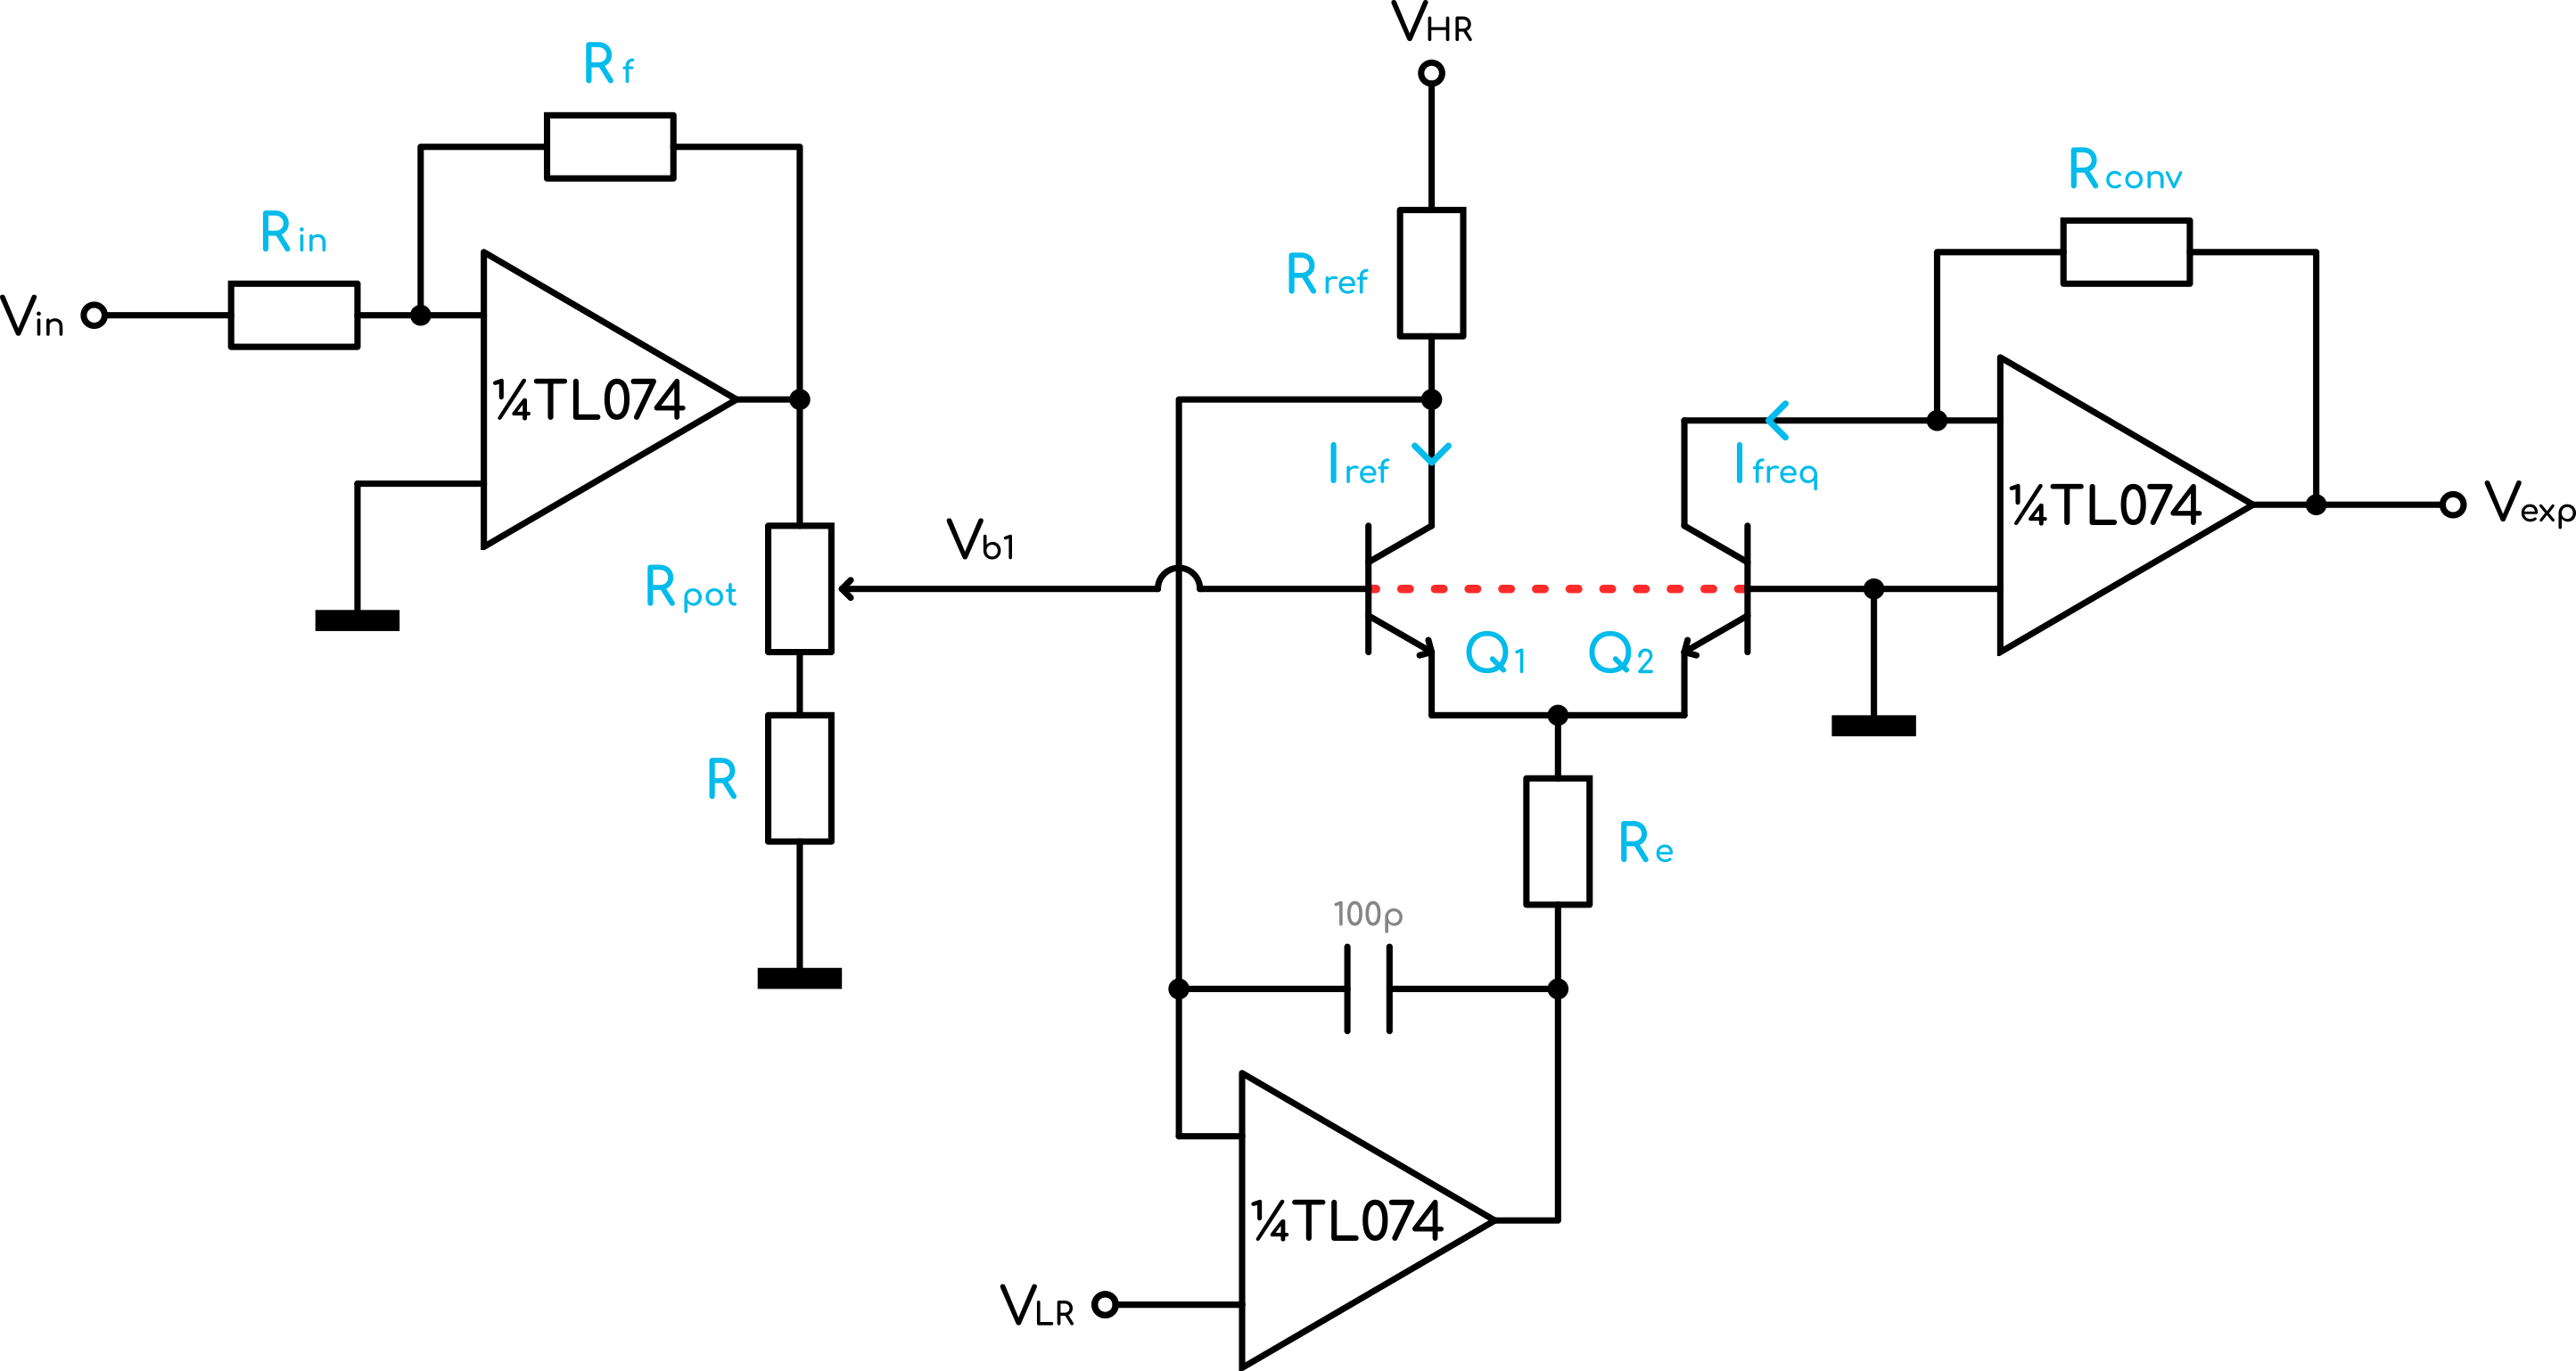
\includegraphics{circuits/exponential_converter_circuit.png}
    \caption{Schema elettrico del convertitore tensione lineare-esponenziale}
    \label{exponential_converter_circuit}
\end{figure}

\begin{displaymath}
    V_{exp}=R_{conv}\cdot \frac{V_{HR}-V_{LR}}{R_{ref}}e^{\left(\frac{s\cdot V_{in}}{V_T}\right)}\ [V]
\end{displaymath}

%--------------------------------------------------------------------------------------------

\subsection*{Dimensionamento e Scelta dei Componenti}

%--------------------------------------------------------------------------------------------

Passiamo quindi al dimensionamento dei componenti, in modo da imporre al circuito il
comportamento voluto.

Come prima cosa calcoliamo il valore del guadagno $s$ dell'amplificatore invertente.
Si vuole:

\begin{displaymath}
    I_{freq}=I_{ref}e^{\left(\frac{s\cdot V_{in}}{V_T}\right)}
    \qquad
    \xrightarrow{+\Delta V_{in}}
    \qquad
    2I_{freq}=I_{ref}e^{\left(\frac{s\cdot(V_{in}+\Delta V_{in})}{V_T}\right)}
\end{displaymath}

qundi un raddoppio della corrente $I_{freq}$ per ogni variazione $\Delta V_{in}=1\ V$.
Allora possiamo riscrivere la relazione nel seguente modo:

\begin{displaymath}
    \frac{2I_{freq}}{I_{freq}}=
    \frac{I_{ref}e^{\left(\frac{s\cdot(V_{in}+\Delta V_{in})}{V_T}\right)}}
    {I_{ref}e^{\left(\frac{s\cdot V_{in}}{V_T}\right)}}
    \
    \rightarrow
    \
    2=e^{\left(\frac{s\cdot\Delta V_{in}}{V_T}\right)}
    \
    \rightarrow
    \
    ln(2)=\frac{s\cdot\Delta V_{in}}{V_T}
    \
    \rightarrow
    \
    s=\frac{V_T\cdot ln(2)}{\Delta V_{in}}
\end{displaymath}

\begin{displaymath}
    s=\frac{26\ mV\cdot 0.6931}{1\ V}\approx0.018\approx\frac{1}{55.5}
\end{displaymath}

\begin{displaymath}
    s=\frac{R_f}{R_{in}}\cdot\frac{\%R_{pot}+R}{R_{pot}+R}
    =\frac{2\ k\Omega}{100\ k\Omega}\cdot\frac{440\ \Omega}{490\ \Omega}
    \approx 0.018
\end{displaymath}

quindi:

\begin{itemize}
    \item $R_f = 2\ k\Omega$;
    \item $R_{in} = 100\ k\Omega$;
    \item $R_{pot} = 100\ \Omega$;
    \item $R = 390\ \Omega$;
\end{itemize}

Scegliamo anche $R_{conv}=3.3\ k\Omega$, per avere come massimo valore di corrente
$I_{freq} = 3\ mA$ ($V_{exp}\approx+10\ V$ in uscita dal convertitore corrente-tensione),
in corrispondenza di una tensione di ingresso $V_{in}=+8\ V$. Da qui possiamo quindi calcolare
il valore di $I_{ref}$:

\begin{displaymath}
    I_{ref}=I_{freq}e^{\left(-\frac{s\cdot V_{in}}{V_T}\right)}
    =0.003e^{\left(-\frac{0.018\cdot8}{0.026}\right)}
    \approx11.8\ \mu A
\end{displaymath}

Impostando quindi $V_{HR}=+12\ V$ e $V_{LR}=0\ V$ calcoliamo $R_{ref}$:

\begin{displaymath}
    R_{ref}=\frac{V_{HR}}{I_{ref}}=\frac{12}{11.8\cdot10^{-6}}\approx 1\ M\Omega
\end{displaymath}

Ora, poichè la corrente massima a scorrere in $R_e$ vale $I_{ref}+I_{freq}\approx3\ mA$
potremmo scegliere anche $R_e=R_{conv}=3.3\ k\Omega$. In questo modo sommando le cadute di
potenziale $V_{R_{ref}}$, $V_{ce\_sat\_1}$ e $V_{R_e}$, saremmo dentro il limite dei valori
di alimentazione, ottenendo $\approx 22.2\ V\ < 24\ V= 2V_{cc}$.

Se però andiamo a calcolare la caduta di potenziale ai capi di $R_e$ corrispondente a $V_{in}=0\ V$,
ovvero:

\begin{displaymath}
    V_{R_e}=R_e(I_{ref}+I_{freq})=3.3\cdot10^3\cdot23.6\cdot10^{-6}\approx77.9\ mV
\end{displaymath}

notiamo che un valore di resistenza maggiore aumenterebbe la linearità del circuito per bassi
livelli di $V_{in}$, in quanto la caduta di potenziale sul resistore ha modulo maggiore e
risulta meno influenzata dal rumore. Si modifica allora il circuito cosicché che la
resistenza di emettitore sia variabile in modo non-lineare, a seconda della corrente
richiesta in uscita. Questo è reso possibile sostituendo ad $R_e$ un parallelo tra due resistori
di diverso valore, di cui quello più piccolo collegato in serie ad un diodo, l'elemento che
si occuperà effettivamente di modificare il valore di resistenza.

\begin{figure}[H]
    \centering
    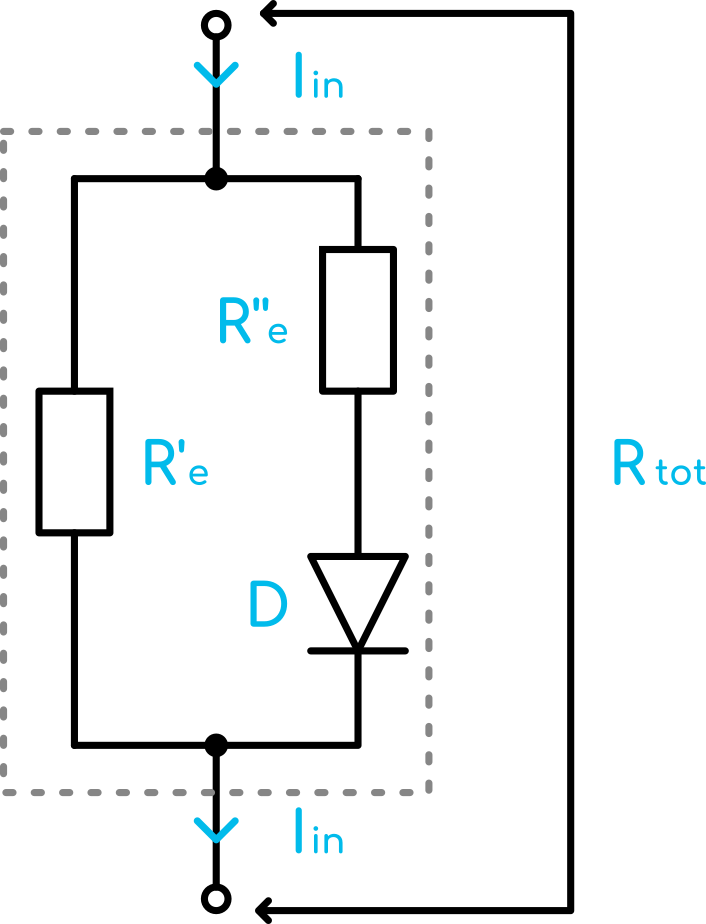
\includegraphics{circuits/Rtot_circuit.png}
    \caption{Schema elettrico del resistore variabile}
    \label{Rtot_circuit}
\end{figure}

Come resistori possiamo scegliere qualsiasi valore, purchè non comporti la saturazione
dell'operazionale e si aggiri comunque attorno al $k\Omega$. Si scelgono $R_e'=10\ k\Omega$
e $R_e''=1.2\ k\Omega$.

\begin{equation*}
    R_{tot} =
    \left\{
    \begin{array}{lr}
        R_e'        & \text{con diodo spento, ovvero } I_{ref}+I_{freq}\leq\frac{V_d}{R_e'} \\
        R_e'//R_e'' & \text{con diodo acceso, ovvero } I_{ref}+I_{freq}>\frac{V_d}{R_e'}
    \end{array}
    \right.
\end{equation*}

Per quanto riguarda i componenti, ancora una volta gli amplificatori operazionali utilizzati
sono dei TL074, mentre si sceglie un MPQ3904 \cite{mpq3904} per i transistor, chip che
ospita 4 unità al proprio interno, e vista la disponibilità, il diodo in figura viene
sostituito con uno dei 4 transistor del chip configurato come diodo.

\begin{figure}[H]
    \centering
    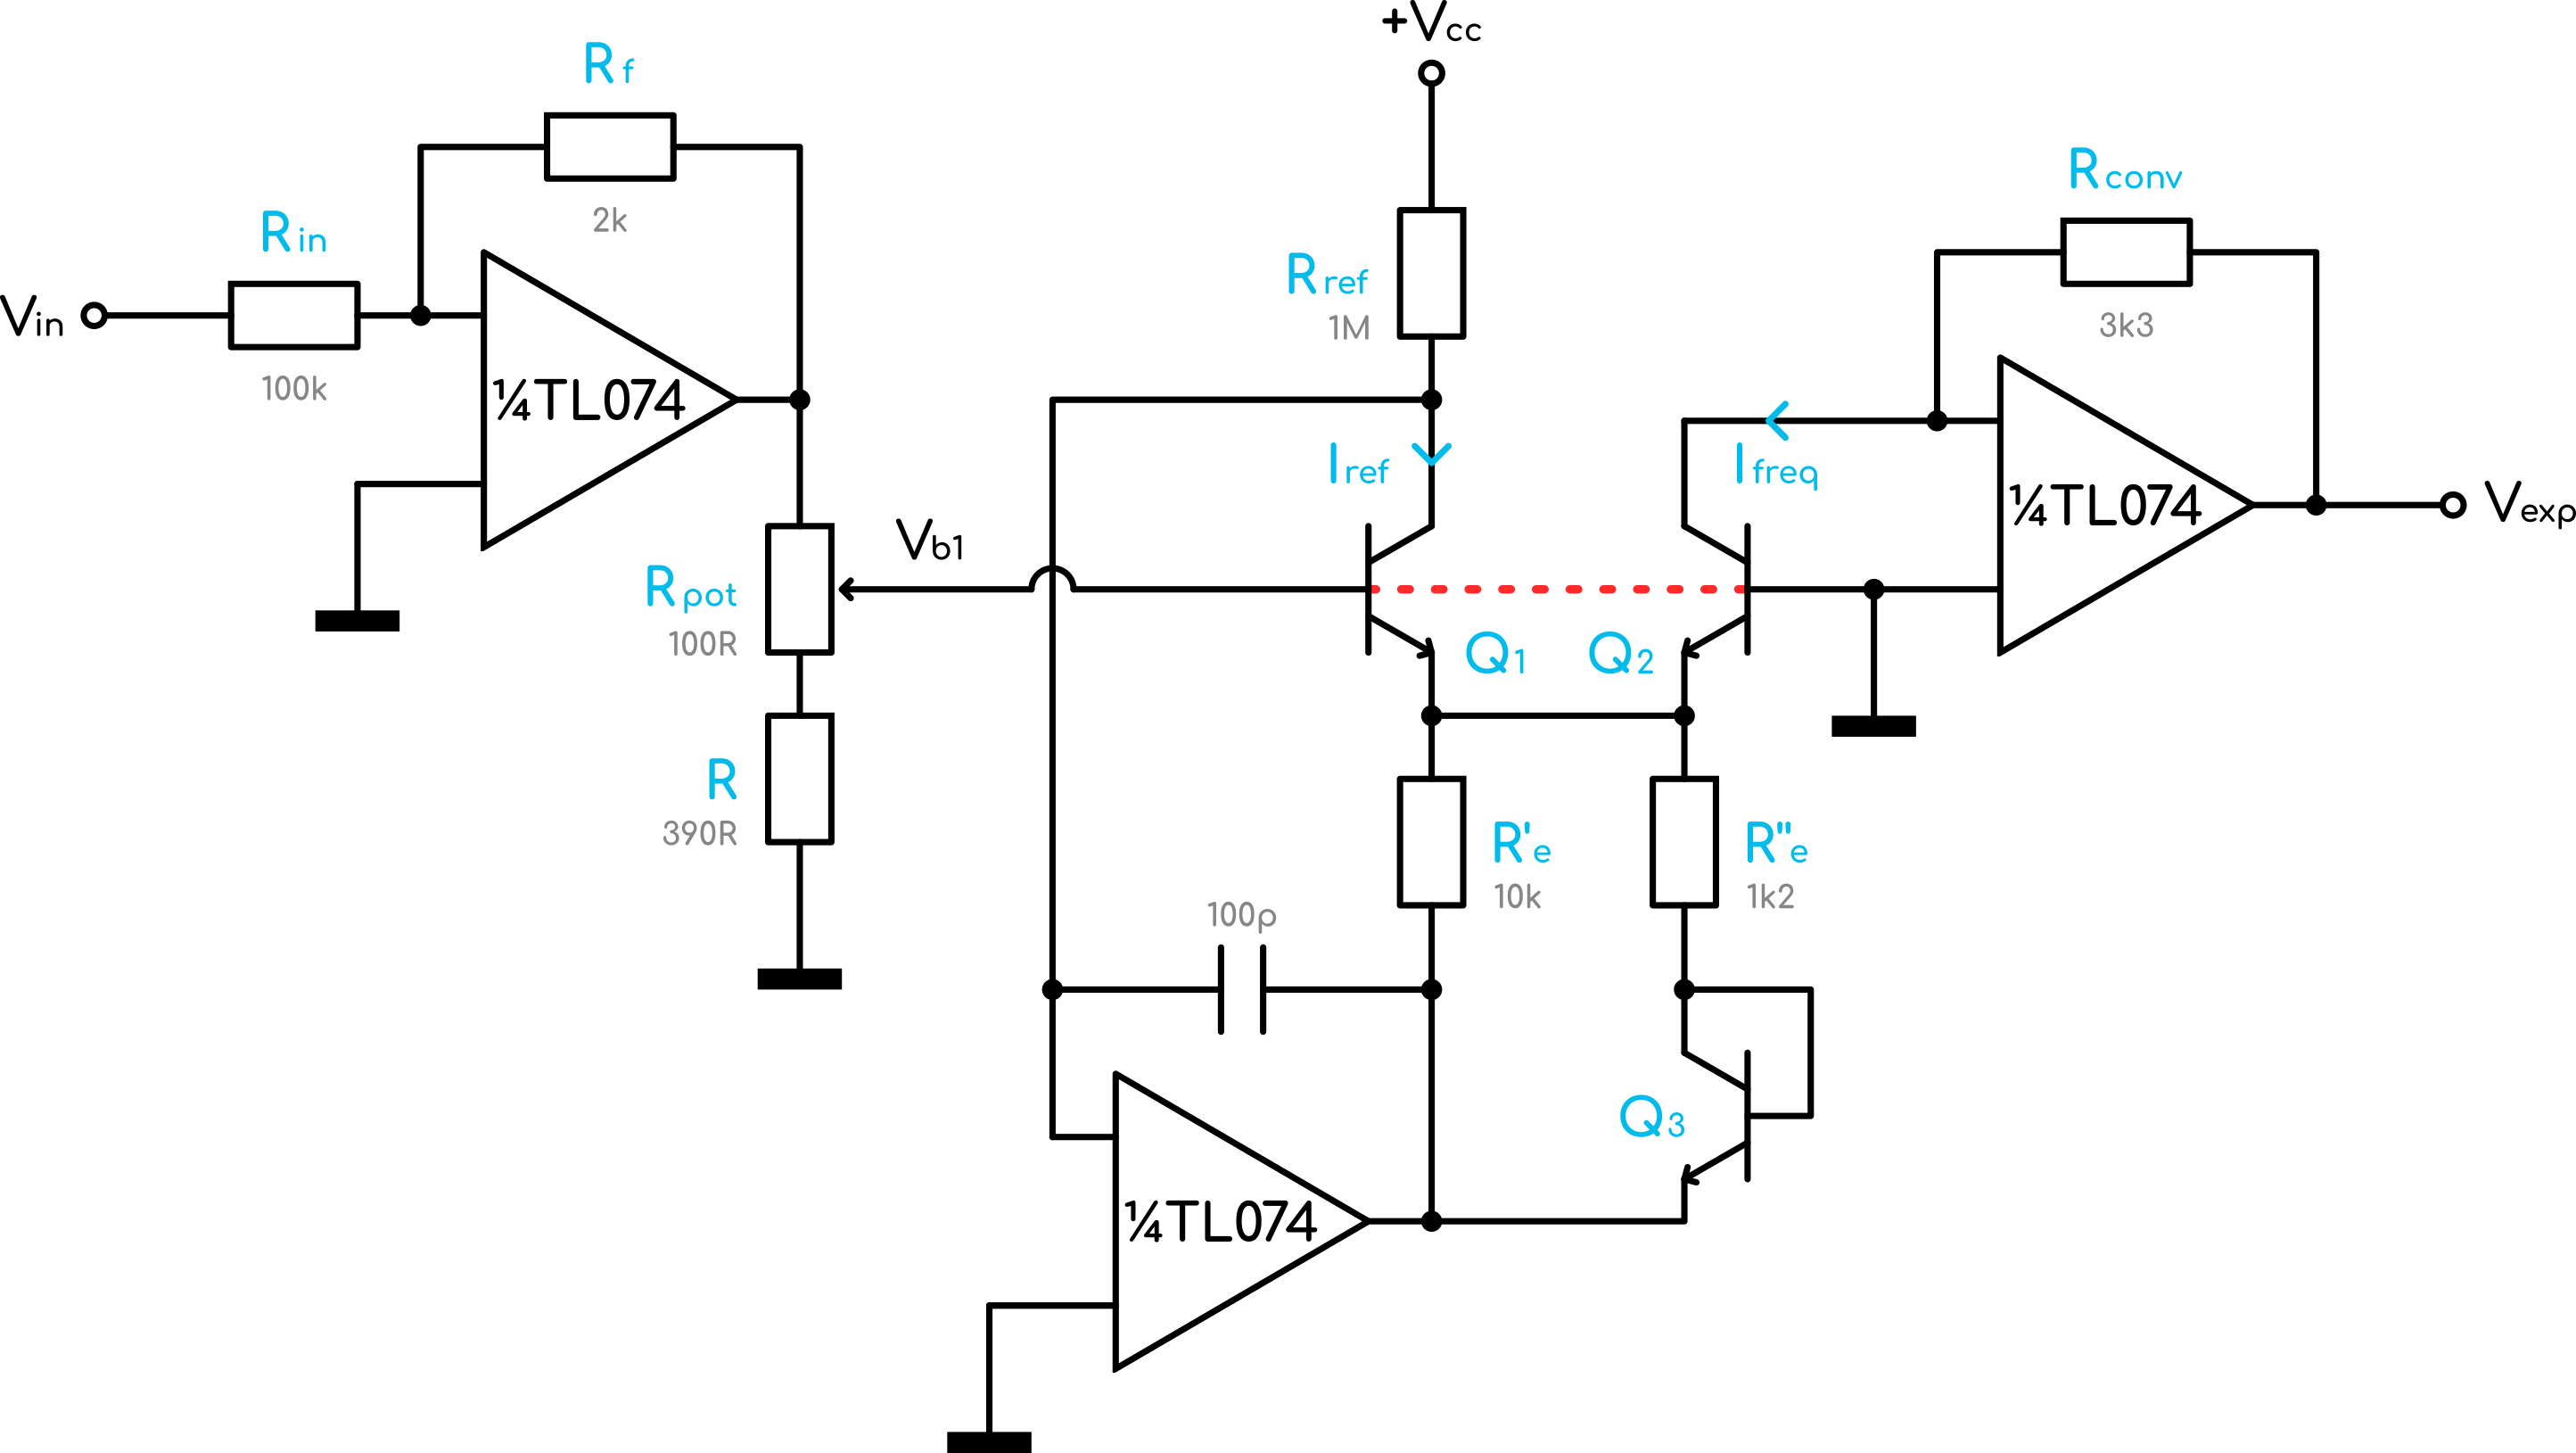
\includegraphics{circuits/complete_exponential_converter_circuit.png}
    \caption{Schema elettrico del convertitore tensione lineare-esponenziale completo}
    \label{complete_exponential_converter_circuit}
\end{figure}

%--------------------------------------------------------------------------------------------

\subsection*{Risultati Pratici e Misure}

%--------------------------------------------------------------------------------------------

Analizziamo ora il comportamento del circuito.

\begin{minipage}[H]{0.3\textwidth}
    \begin{table}[H]
        \centering
        \csvreader[
            before reading = \footnotesize\sisetup{round-mode = places,}
            \setlength{\tabcolsep}{2.5pt},
            tabular = |c|c|c|c|,
            table head = \hline $V_{in}$ & $V_{attesa}$ & $V_{exp}$ & $V_{opamp}$ \\\hline,
            late after line = \\\hline,
        ]{data/misure_Re_low_gain.csv}{}{
            \csvcoli & \csvcolii & \csvcoliii & \csvcoliv
        }
        \caption{test}
        \label{expo1}
    \end{table}
\end{minipage}
\begin{minipage}[H]{0.35\textwidth}
    \begin{figure}[H]
        \centering
        \begin{tikzpicture}[scale = 0.65]
            \begin{semilogyaxis}[
                    title = Transcaratteristica,             % title
                    no marks,
                    xmin = 0, xmax = 12,            % limit values
                    ymin = 0.01, ymax = 50,
                    grid = major,                   % grid
                    grid style = {dashed, gray!30},
                    xlabel = $V_{in}$,              % axis titles and units
                    ylabel = $V_{exp}$,
                    x unit = \si{\V}, y unit = \si{\V},
                    legend style = {at = {(0.5, -0.25)}, anchor = north},
                    cycle list name = modular,
                ]

                \addplot
                table[x = vin, y = vattesa, col sep = comma]{./data/misure_Re_low_gain.csv};

                \addplot
                table[x = vin, y = vexpo, col sep = comma]{./data/misure_Re_low_gain.csv};

                \legend{Calcolato, Misurato}
            \end{semilogyaxis}
        \end{tikzpicture}

        \caption{test}
        \label{testgraph}
    \end{figure}
\end{minipage}
\begin{minipage}[H]{0.35\textwidth}
    \begin{figure}[H]
        \centering
        \begin{tikzpicture}[scale = 0.65]
            \begin{semilogyaxis}[
                    title = Transcaratteristica,             % title
                    no marks,
                    xmin = 0, xmax = 12,            % limit values
                    ymin = 0.01, ymax = 50,
                    grid = major,                   % grid
                    grid style = {dashed, gray!30},
                    xlabel = $V_{in}$,              % axis titles and units
                    ylabel = $V_{exp}$,
                    x unit = \si{\V}, y unit = \si{\V},
                    legend style = {at = {(0.5, -0.25)}, anchor = north},
                    cycle list name = modular,
                ]

                \addplot
                table[x = vin, y = vattesa, col sep = comma]{./data/misure_Re_low_gain.csv};

                \addplot
                table[x = vin, y = vexpo, col sep = comma]{./data/misure_Re_low_gain.csv};

                \legend{Calcolato, Misurato}
            \end{semilogyaxis}
        \end{tikzpicture}

        \caption{test}
        \label{testgraph2}
    \end{figure}
\end{minipage}

%--------------------------------------------------------------------------------------------

\section{Somma di più Ingressi}

%--------------------------------------------------------------------------------------------

TODO descrizione sommatore

%--------------------------------------------------------------------------------------------

\section{Clipper}

%--------------------------------------------------------------------------------------------

TODO descrizione clipper

%--------------------------------------------------------------------------------------------

\subsection*{Risultati Pratici e Misure}

%--------------------------------------------------------------------------------------------

TODO misure e acquisizioni clipper

%--------------------------------------------------------------------------------------------
